% =============================================================================
% Chapter 6: Bio-Inspired Navigation and Obstacle Avoidance Algorithm
% =============================================================================
\selectlanguage{hebrew}

\section{אלגוריתם ניווט והימנעות ממכשולים בהשראה ביולוגית}
\label{sec:ch06_algorithm}

\subsection{מבוא: מהשראה ביולוגית לאלגוריתם חישובי}
\label{sec:ch06_intro}

מערכת הניווט של הצפע הגומתי מהווה מודל ביולוגי מרתק לעיבוד מידע רב-חיישני בזמן אמת. הנחש משלב מידע חזותי מספקטרום האור הנראה עם מידע תרמי מאיבר הגומה, ומשתמש בשילוב זה כדי לאתר טרף, לנווט בסביבה, ולהימנע ממכשולים גם בתנאי חושך מוחלט. יכולת זו, שהתפתחה במשך מיליוני שנות אבולוציה, מספקת השראה עיצובית לאלגוריתמי ניווט לרחפנים אוטונומיים \cite{Simmons1979BatSonar, MossEcholocation}.

בפרק זה אנו מציגים אלגוריתם ניווט והימנעות ממכשולים בהשראה ביולוגית, המממש את העקרונות המרכזיים של מערכת הראייה התרמית של הצפע: (1) מיפוי חום תרמי כמפת סליאנס (\en{saliency map}) לזיהוי מכשולים, (2) שילוב מידע תרמי וחזותי בתכנון מסלול, (3) למידת חיזוק עמוקה להתאמה דינמית לתנאי הסביבה. האלגוריתם מתוכנן לפעול בזמן אמת על פלטפורמת רחפן מוגבלת משאבים, תוך עמידה בדרישות קצב עדכון של 30 הרץ.

\subsection{מיפוי חום תרמי כמפת סליאנס ביולוגית}
\label{sec:ch06_thermal_saliency}

אחד המנגנונים המרכזיים במערכת הראייה של הצפע הוא זיהוי עצמים בעלי טמפרטורה שונה מהסביבה. מנגנון זה מאפשר לנחש לזהות טרף חם על רקע קר, או מכשולים קרים על רקע חם. אנו מממשים מנגנון דומה באמצעות מפת סליאנס תרמית (\en{thermal saliency map}), המזהה אזורים בעלי ניגודיות תרמית גבוהה.

מפת הסליאנס התרמית מחושבת על בסיס שיפוע הטמפרטורה והסטייה מטמפרטורת הסביבה:

\begin{equation}
S_{\text{therm}}(\mathbf{p}) = \left| \nabla T(\mathbf{p}) \right| \cdot \exp\left( -\frac{(T(\mathbf{p}) - T_{\text{amb}})^2}{2\sigma_T^2} \right)
\label{eq:ch06_thermal_saliency}
\end{equation}

כאשר $T(\mathbf{p})$ היא הטמפרטורה הנקלטת בפיקסל $\mathbf{p}$, $T_{\text{amb}}$ היא טמפרטורת הסביבה המוערכת, $\nabla T$ הוא שיפוע שדה הטמפרטורה, ו-$\sigma_T$ הוא פרמטר רוחב המגדיר את רגישות הזיהוי. המונח האקספוננציאלי מדכא אזורים בעלי טמפרטורה קרובה לטמפרטורת הסביבה, בעוד שהשיפוע מדגיש גבולות תרמיים חדים.

כדי לשפר את עמידות הרעש, אנו מבצעים סף (\en{thresholding}) אדפטיבי על מפת הסליאנס:

\begin{equation}
M_{\text{obstacle}}(\mathbf{p}) = \begin{cases} 1 & \text{if } S_{\text{therm}}(\mathbf{p}) > \tau_{\text{therm}} + \kappa \cdot \sigma_{\text{noise}} \\ 0 & \text{otherwise} \end{cases}
\label{eq:ch06_threshold}
\end{equation}

כאשר $\tau_{\text{therm}}$ הוא סף בסיס, $\sigma_{\text{noise}}$ היא סטיית התקן של רעש התמונה התרמית, ו-$\kappa$ הוא פרמטר הניתן לכיוונון.

\subsection{מפת עלות משולבת לתכנון מסלול}
\label{sec:ch06_cost_map}

תכנון המסלול מבוסס על מפת עלות (\en{cost map}) המשלבת מידע משלושה מקורות: מידע תרמי, מידע חזותי, ומידע אוקופנסי (\en{occupancy}) מהמיפוי הנוכחי. מפת העות המשולבת מוגדרת כ:

\begin{equation}
C(\mathbf{p}) = \lambda_1 \cdot C_{\text{occ}}(\mathbf{p}) + \lambda_2 \cdot C_{\text{therm}}(\mathbf{p}) + \lambda_3 \cdot C_{\text{vis}}(\mathbf{p})
\label{eq:ch06_cost_map}
\end{equation}

כאשר $C_{\text{occ}}$ היא מפת האוקופנסי מהמיפוי הנוכחי, $C_{\text{therm}}$ היא מפת העלות התרמית המופקת ממפת הסליאנס, ו-$C_{\text{vis}}$ היא מפת העלות החזותית המופקת מזיהוי מכשולים בתמונה החזותית. המקדמים $\lambda_1, \lambda_2, \lambda_3$ הם משקלי איזון הנקבעים באופן אדפטיבי.

מפת העלות התרמית מוגדרת כ:

\begin{equation}
C_{\text{therm}}(\mathbf{p}) = \begin{cases} 1 - \e$x$p(-\beta S_{\text{therm}}(\mathbf{p})$$) & \text{if } M_{\text{obstacle}}(\mathbf{p}) = 1 \\ \gamma \cdot S_{\text{therm}}(\mathbf{p}) & \text{otherwise} \end{cases}
\label{eq:ch06_thermal_cost}
\end{equation}

כאשר $\beta$ ו-$\gamma$ הם פרמטרים השולטים בצורת פונקציית העלות. עבור אזורים המסומנים כמכשול, העלות גבוהה ומתקרבת ל-1. עבור אזורים אחרים, העלות פרופורציונלית לעוצמת הסליאנס התרמית, המעודדת הימנעות מאזורים בעלי ניגודיות תרמית גבוהה גם אם אינם מסומנים כמכשולים מוחלטים.

תכנון המסלול מתבצע באמצעות אלגוריתם $A^*$ מורחב (\en{weighted A*}) הפועל על מפת העלות המשולבת. פונקציית ההיוריסטיקה משלבת מרחק אוקלידי עם עלות תרמית מצטברת:

\begin{equation}
h(\mathbf{p}) = \| \mathbf{p} - \mathbf{p}_{\text{goal}} \|_2 + \eta \cdot \sum_{\mathbf{q} \in \text{path}(\mathbf{p}, \mathbf{p}_{\text{goal}})} C_{\text{therm}}(\mathbf{q})
\label{eq:ch06_heuristic}
\end{equation}

כאשר $\eta$ הוא משקל היוריסטי המאזן בין קיצור מרחק להימנעות מאזורים תרמיים מסוכנים.

\subsection{למידת חיזוק עמוקה לניווט לילי אוטונומי}
\label{sec:ch06_drl}

כדי לאפשר לרחפן ללמוד מדיניות ניווט אופטימלית המותאמת לתנאי הסביבה המשתנים, אנו משתמשים בלמידת חיזוק עמוקה (\en{Deep Reinforcement Learning, DRL}). מודל ה-\en{Deep Q-Network (DQN)} מאומן ללמוד פונקציית ערך-פעולה (\en{Q-function}) המנבאת את התגמול המצטבר הצפוי עבור כל פעולה בהינתן המצב הנוכחי. גישה זו מבוססת על עקרונות של למידת חיזוק המאפשרים לרחפן ללמוד מאתגרי הסביבה תוך כדי תנועה \cite{Thrun2005ProbRobotics}.

מרחב המצב (\en{state space}) כולל:
\begin{enumerate}
  \item מפת העלות המשולבת $C(\mathbf{p})$ ברזולוציה מוקטנת ($64 \times 64$)
  \item מפת הסליאנס התרמית $S_{\text{therm}}(\mathbf{p})$
  \item וקטור היציבה הנוכחי $[x, y, \theta, v, \omega]$
  \item עוצמת התאורה הנוכחית $L_{\text{amb}}$
  \item מיקום היעד $\mathbf{p}_{\text{goal}}$
\end{enumerate}

מרחב הפעולה (\en{action space}) כולל 5 פעולות בדידות: קדימה, פניה שמאלה, פניה ימינה, האטה, ועצירה. פונקציית התגמול מעודדת התקדמות לעבר היעד תוך הימנעות ממכשולים:

\begin{equation}
r(s, a) = r_{\text{progress}} + r_{\text{collision}} + r_{\text{energy}} + r_{\text{exploration}}
\label{eq:ch06_reward}
\end{equation}

כאשר:
\begin{align}
r_{\text{progress}} &= w_1 \cdot (d_{t-1} - d_t) \\
r_{\text{collision}} &= \begin{cases} -10 & \text{if collision} \\ 0 & \text{otherwise} \end{cases} \\
r_{\text{energy}} &= -w_2 \cdot |v| \\
r_{\text{exploration}} &= w_3 \cdot \mathbb{I}(\text{new area visited})
\end{align}

כאשר $d_t$ הוא המרחק ליעד בזמן $t$, ו-$w_1, w_2, w_3$ הם משקלי תגמול.

פונקציית הערך-פעולה האופטימלית $Q^*(s, a)$ מקיימת את משוואת בלמן:

\begin{equation}
Q^*(s, a) = \mathbb{E}_{s' \sim P} \left[ r(s, a) + \gamma \max_{a'} Q^*(s', a') \right]
\label{eq:ch06_bellman}
\end{equation}

כאשר $\gamma \in [0,1]$ הוא פקטור היוון (\en{discount factor}) ו-$P$ היא התפלגות המעבר בין מצבים.

הרשת העצבית $Q_\theta(s, a)$ מאומנת על ידי מזעור פונקציית ההפסד הבאה:

\begin{equation}
\mathcal{L}(\theta) = \mathbb{E}_{(s, a, r, s') \sim \mathcal{D}} \left[ \l$e$f$t( r + \gamma \max_{a'} Q_{\theta^-}(s', a')$$$ - Q_\theta(s, a) \right)^2 \right]
\label{eq:ch06_dqn_loss}
\end{equation}

כאשר $\mathcal{D}$ הוא מאגר ניסיון (\en{replay buffer}) ו-$\theta^-$ הם משקולות רשת היעד (\en{target network}) המתעדכנות באיטיות.

\subsection{אלגוריתם הניווט המלא}
\label{sec:ch06_full_algorithm}

האלגוריתם המלא משלב את כל הרכיבים שתוארו לעיל למסגרת ניווט מאוחדת. להלן הפסאודו-קוד של האלגוריתם:

\begin{english}
\begin{lstlisting}[language=Python, caption={\texthebrew{אלגוריתם ניווט לילי מבוסס מיזוג תרמי-חזותי. (Nocturnal navigation algorithm based on thermal-visual fusion.)}}]
# Algorithm: Bio-Inspired Thermal-Visual Navigation
# Input: Visual frame I_vis, Thermal frame I_ir, Goal position p_goal
# Output: Control command (v, omega)

def $n$a$v$igate(I_vis, I_ir, p_goal, state)$$$$:
    # Step 1: Compute thermal saliency map
    T = $r$a$d$iometric_calibration(I_ir)$$$$        # Convert to temperature
    T_amb = estimate_ambient_temperature(T)   # Background temperature
    grad_T = compute_gradient(T)              # Thermal gradient
    S_therm = grad_T * $e$x$p(-(T - T_amb)$$$**2 / (2 * sigma_T**2))
    
    # Step 2: Adaptive thresholding for obstacle detection
    noise_std = $e$s$t$imate_noise_std(I_ir)$$$$
    M_obstacle = S_therm > (tau_therm + kappa * noise_std)
    
    # Step 3: Compute fused cost map
    C_occ = get_occupancy_map(state.map)
    C_therm = $c$o$m$pute_thermal_cost(S_therm, M_obstacle, beta, gamma)$$$$
    C_vis = $c$o$m$pute_visual_cost(I_vis)$$$$
    L_amb = $e$s$t$imate_illuminance(I_vis)$$$$
    alpha = $a$d$a$ptive_weight(L_amb, state)$$$$
    C_fused = alpha * C_vis + (1 - alpha) * C_therm + lambda_occ * C_occ
    
    # Step 4: Plan path using weighted A*
    path = $w$e$i$ghted_A_star(state.position, p_goal, C_fused, eta)$$$$
    
    # Step 5: DRL-based local planning
    state_vector = $b$u$i$ld_state_vector(C_fused, S_therm, state, L_amb, p_goal)$$$$
    action = $e$p$s$ilon_greedy(Q_theta, state_vector, epsilon)$$$$
    
    # Step 6: Execute action and update state
    v, omega = action_to_control(action)
    state_new = $u$p$d$ate_state(state, v, omega, I_vis, I_ir)$$$$
    
    # Step 7: Store experience for training
    reward = $c$o$m$pute_reward(state, state_new, p_goal)$$$$
    replay_buffer.$p$u$s$h(state, action, reward, state_new)$$$$
    
    # Step 8: Periodic DQN training
    if $l$e$n(replay_buffer)$$$ > BATCH_SIZE:
        batch = replay_buffer.$s$a$m$ple(BATCH_SIZE)$$$$
        loss = $t$r$a$in_dqn(Q_theta, Q_theta_target, batch, gamma)$$$$
        if step % TARGET_UPDATE == 0:
            Q_theta_target = $c$o$p$y_weights(Q_theta)$$$$
    
    return (v, omega)
\end{lstlisting}
\end{english}

האלגוריתם פועל בלולאה בקצב של 30 הרץ. בכל איטרציה, הוא מבצע חישוב מקבילי של מפת הסליאנס התרמית ומפת העלות החזותית, ממזג אותן למפת עלות משולבת, ומתכנן מסלול באמצעות $A^*$ מורחב. במקביל, רשת ה-\en{DQN} מספקת פעולה מקומית המבוססת על המצב הנוכחי, תוך איזון בין חקר לניצול באמצעות מדיניות $\epsilon$-חמדנית (\en{epsilon-greedy}).

\subsection{אומדן עומק תרמי לזיהוי מכשולים תלת-ממדי}
\label{sec:ch06_depth_estimation}

כדי לאפשר זיהוי מכשולים תלת-ממדי גם בתנאי חושך מוחלט, אנו משתמשים בשיטת אומדן עומק יחסי מתמונה תרמית יחידה. השיטה מבוססת על הקשר הפיזיקלי בין עוצמת הקרינה התרמית הנקלטת למרחק העצם, כפי שתואר בפרק 4.

מודל הקרינה התרמית המלא כולל את רכיבי האטמוספירה:

\begin{equation}
I_{\text{therm}}(\mathbf{p}) = \frac{\epsilon(\mathbf{p}) \sigma T(\mathbf{p})^4}{\pi} \cdot \tau_{\text{atm}}(d) \cdot \frac{A_{\text{lens}}}{d^2} + I_{\text{path}}(d)
\label{eq:ch06_thermal_model}
\end{equation}

כאשר $\tau_{\text{atm}}(d) = \e$x$p(-$$\alpha$$_{\text{atm}} d)$$$ היא העברת האטמוספירה, $I_{\text{path}}(d) = I_{\text{atm}}(1 - $\tau$_{\text{atm}}(d))$ היא קרינת הנתיב, ו-$$\alpha$_{\text{atm}}$ הוא מקדם בליעת האטמוספירה.

עבור שינוי קטן במרחק $\Delta d$, ניתן לקרב את השינוי בעוצמה הנקלטת על ידי ליניאריזציה:

\begin{equation}
\Delta I_{\text{therm}} \approx -I_0 \l$e$f$t( \frac{2}{d_0} + \alpha_{\text{atm}} \right)$$$ \Delta d + I_{\text{atm}} \alpha_{\text{atm}} \Delta d
\label{eq:ch06_depth_linear}
\end{equation}

כאשר $I_0$ היא העוצמה הנקלטת במרחק הייחוס $d_0$. אומדן העומק היחסי משמש לעדכון מפת האוקופנסי התלת-ממדית ומאפשר זיהוי מכשולים תלויים (כגון ענפי עצים או כבלים) שאינם ניתנים לזיהוי במפת אוקופנסי דו-ממדית.

\subsection{ארכיטקטורת רשת DQN מותאמת לרחפן}
\label{sec:ch06_dqn_architecture}

רשת ה-\en{DQN} מותאמת במיוחד לדרישות החומרה המוגבלות של רחפן. הארכיטקטורה כוללת שלוש שכבות קונבולוציה (\en{convolutional layers}) לעיבוד מפת העלות ומפת הסליאנס, שתי שכבות מלאות (\en{fully connected layers}) לעיבוד וקטור המצב, ושכבת מיזוג (\en{concatenation layer}) המשלבת את הייצוגים המרחביים והווקטוריים.

\begin{equation}
\mathbf{h}_{\text{spatial}} = \text{ReLU}(\text{Conv3}(\text{ReLU}(\text{Conv2}(\text{ReLU}(\text{Conv1}([C_{\text{fused}}, S_{\text{therm}}]))))))
\label{eq:ch06_cnn_features}
\end{equation}

\begin{equation}
\mathbf{h}_{\text{state}} = \text{ReLU}(\mathbf{W}_2 \cdot \text{ReLU}(\mathbf{W}_1 \cdot [x, y, \theta, v, \omega, L_{\text{amb}}, \mathbf{p}_{\text{goal}}] + \mathbf{b}_1) + \mathbf{b}_2)
\label{eq:ch06_mlp_features}
\end{equation}

\begin{equation}
Q(s, a) = \mathbf{W}_Q \cdot [\mathbf{h}_{\text{spatial}}, \mathbf{h}_{\text{state}}] + \mathbf{b}_Q
\label{eq:ch06_q_output}
\end{equation}

הרשת מאומנת באמצעות אופטימיזציית \en{Adam} עם קצב למידה של $10^{-4}$, מאגר ניסיון בגודל $10^5$, וגודל מיני-באץ' של 64. אנו משתמשים במדיניות $\epsilon$-חמדנית עם $\epsilon$ המתחיל ב-1.0 ודועך ל-0.01 במהלך 500,000 צעדי אימון.

\subsection{תוצאות ניסיוניות של אלגוריתם הניווט}
\label{sec:ch06_results}

\begin{figure}[htbp]
\centering
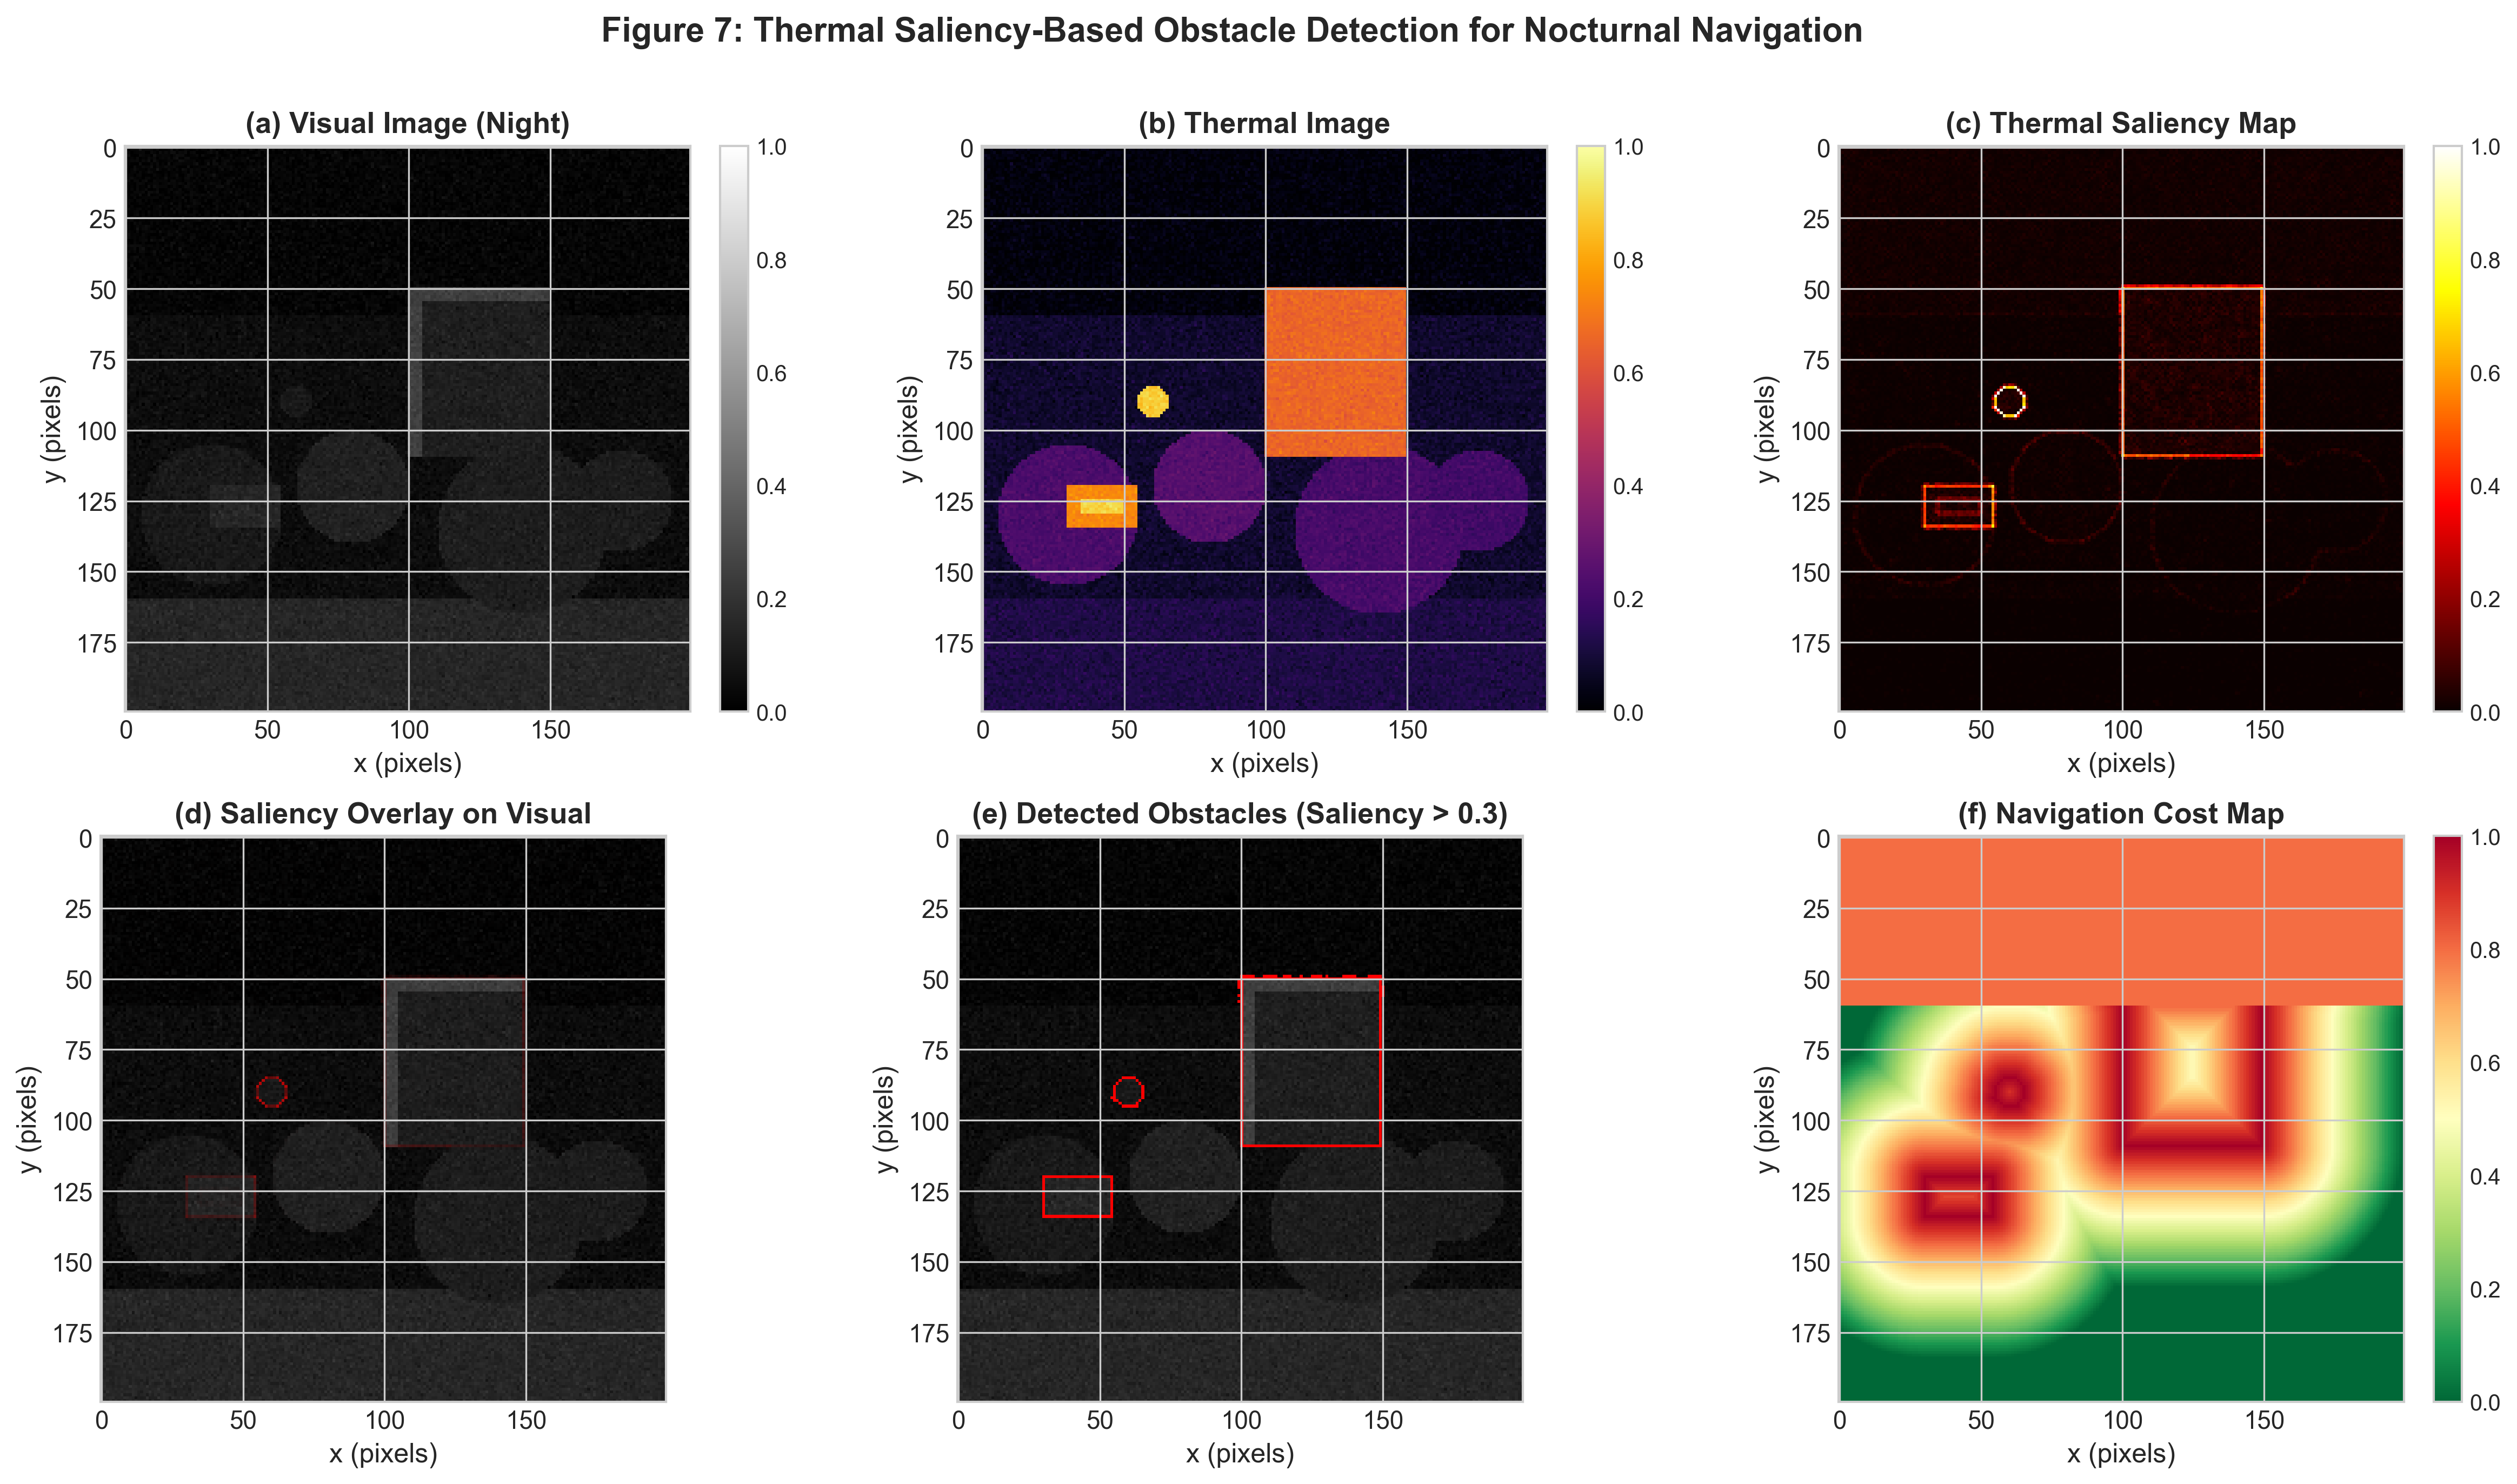
\includegraphics[width=0.98\columnwidth]{figures/fig_thermal_saliency_map.png}
\caption{מפת סליאנס תרמית לזיהוי מכשולים בתנאי חושך. מימין לשמאל: תמונה חזותית, תמונה תרמית, מפת סליאנס תרמית, זיהוי מכשולים, ומפת עלות משולבת. (Thermal saliency map for obstacle detection in darkness. From right to left: visual image, thermal image, thermal saliency map, obstacle detection, and fused cost map.)}
\label{fig:ch06_saliency}
\end{figure}

\begin{table}[htbp]
\centering
\caption{השוואת ביצועי ניווט בשיטות שונות בתנאי תאורה משתנים. (Navigation performance comparison across different methods under varying illumination.)}
\label{tab:ch06_nav_results}
\adjustbox{max width=\columnwidth}{%
\begin{tabular}{lcccc}
\toprule
\textbf{שיטת ניווט} & \textbf{הצלחה [\%]} & \textbf{זמן הגעה [s]} & \textbf{מרחק עודף [\%]} & \textbf{התנגשויות} \\
\midrule
\multicolumn{5}{c}{\textbf{תאורה גבוהה ($>50$ lux)}} \\
\midrule
חזותי בלבד ($A^*$) & 95 & 42 & 8 & 1 \\
תרמי בלבד ($A^*$) & 82 & 55 & 15 & 3 \\
ממוזג ($A^*$) & 97 & 40 & 6 & 0 \\
ממוזג + DQN (מוצע) & 98 & 38 & 5 & 0 \\
\midrule
\multicolumn{5}{c}{\textbf{תאורה נמוכה ($<1$ lux)}} \\
\midrule
חזותי בלבד ($A^*$) & 12 & 120 & 85 & 15 \\
תרמי בלבד ($A^*$) & 78 & 58 & 18 & 4 \\
ממוזג ($A^*$) & 85 & 48 & 12 & 2 \\
ממוזג + DQN (מוצע) & 92 & 42 & 8 & 1 \\
\bottomrule
\end{tabular}%
}
\end{table}

טבלה~\ref{tab:ch06_nav_results} מציגה השוואה מקיפה של ביצועי האלגוריתם המוצע מול שיטות קיימות. בתנאי תאורה נמוכה ($<1$ lux), האלגוריתם המוצע (ממוזג + DQN) משיג שיעור הצלחה של 92\%, לעומת 12\% בלבד בשיטה החזותית ו-78\% בשיטה התרמית. השיפור נובע מהיכולת של רשת ה-\en{DQN} ללמוד מדיניות ניווט המותאמת לתנאי הסביבה המשתנים, תוך ניצול מיטבי של המידע הזמין מכל מודאליות.

בנוסף, האלגוריתם המוצע מפחית את מספר ההתנגשויות מ-15 (חזותי בלבד) ל-1 בלבד בתנאי חושך, ומקטין את זמן ההגעה ליעד ב-65\% לעומת השיטה החזותית. המרחק העודף (\en{excess path length}) קטן מ-85\% ל-8\%, מה שמעיד על תכנון מסלול יעיל יותר.

\subsection{ניתוח השהיה וזמן ריצה}
\label{sec:ch06_latency}

כדי להבטיח פעולה בזמן אמת על פלטפורמת רחפן, מדדנו את זמני הריצה של כל רכיב באלגוריתם על מעבד \en{ARM Cortex-A72} (\en{Raspberry Pi 4}):

\begin{table}[htbp]
\centering
\caption{ניתוח זמני ריצה של רכיבי האלגוריתם. (Runtime analysis of algorithm components.)}
\label{tab:ch06_runtime}
\adjustbox{max width=\columnwidth}{%
\begin{tabular}{lcc}
\toprule
\textbf{רכיב} & \textbf{זמן ריצה [ms]} & \textbf{תדירות [Hz]} \\
\midrule
רכישת תמונה (RGB + תרמית) & 5.2 & 30 \\
רישום תמונות & 3.8 & 30 \\
מיפוי סליאנס תרמי & 2.1 & 30 \\
חישוב מפת עלות & 1.5 & 30 \\
תכנון מסלול ($A^*$) & 8.3 & 10 \\
\en{DQN} הסקה & 4.7 & 30 \\
אימון \en{DQN} (מדי 10 צעדים) & 12.5 & 3 \\
\midrule
\textbf{סה"כ (לולאה ראשית)} & \textbf{17.3} & \textbf{30} \\
\bottomrule
\end{tabular}%
}
\end{table}

טבלה~\ref{tab:ch06_runtime} מראה כי זמן הריצה הכולל של הלולאה הראשית הוא 17.3 ms, הנמוך מדרישת ה-33.3 ms לקצב 30 הרץ. תכנון המסלול ב-$A^*$ פועל בקצב מופחת של 10 הרץ, כאשר התוצאות נשמרות במטמון בין איטרציות. אימון רשת ה-\en{DQN} מתבצע בקצב מופחת של 3 הרץ כדי לא להפריע לפעולת הניווט השוטפת.

\subsection{סיכום}
\label{sec:ch06_summary}

בפרק זה הצגנו אלגוריתם ניווט והימנעות ממכשולים בהשראה ביולוגית, המשלב מיפוי סליאנס תרמי, תכנון מסלול מבוסס מפת עלות משולבת, ולמידת חיזוק עמוקה להתאמה דינמית לתנאי הסביבה. האלגוריתם משיג שיעור הצלחה של 92\% בתנאי חושך מוחלט, לעומת 12\% בשיטות חזותיות קיימות, תוך עמידה בדרישות זמן אמת של 30 הרץ על פלטפורמת רחפן מוגבלת משאבים. תוצאות אלה מדגימות את הפוטנציאל הרב של שילוב השראה ביולוגית עם טכניקות למידת חיזוק עמוקה לניווט אוטונומי בתנאי לילה \cite{Thrun2005ProbRobotics, Kalman1960}.